\chapter{Implicações para aprendizagem científica}

O desenvolvimento da computação e o amadurecimento da noção de pensamento computacional traz consigo várias implicações e oportunidades educacionais.

De partida, pode-se dizer que a efetivação do uso do computador como ferramenta para resolução de problemas exige a formação de capital humano. Normalmente, espera-se que estudantes tenham acesso à universidade para introdução das primeiras noções de programação e ciência da computação. Sabe-se contudo que eles se mostram cada vez familiarizados com \textit{smartphones} e outros dispositivo computacionais. Por isso podemos nos perguntar: por que não antecipar essa instrumentalização? 

Esse questionamento se torna ainda mais pertinente em face do percentual reduzido de portadores de grau universitário. A demanda por profissionais com experiência na resolução de problemas computacionais tem crescido numa proporção superior a que academia tem formado. Esse desequilíbrio tem levado grandes empresas de tecnologia como o Google e IBM a dispensar a formação universitária como pre-requisito para contratação \cite{Purtill}.

A motivação para essa antecipação não é apenas de caráter laboral. Como discutiremos ao longo desse capítulo o uso de computadores e do pensamento computacional oferece excelentes contextos para desenvolvimento de competências científicas. O reverso também é verdadeiro: problemas científicos e matemáticos são domínios excelentes para a aplicação e exercício do pensamento computacional. É nessa tese que esse trabalho se apoia. 

No capítulo \ref{pensamento-computacional} mostramos o como conceitos de abstração, decomposição de problemas e simulação, aliados a praticas de representação de problemas se estruturam em torno do pensamento computacional. Ao mesmo tempo que são centrais na ciência do computação, estes elementos também são fundamentais para o desenvolvimento de modelos e para a compreensão e resolução de problemas num largo espectro de disciplinas matemáticas e científicas \cite{Sengupta2013}.

% Soloway argumenta que aprender a programar corresponde a aprender construir mecanismos e explicações. Portanto a capacidade de construir modelos computacionais por programação corresponde a 

A literatura tem demonstrado de diversas formas o como a aprendizagem de programação - uma das praticas de representação - em conjunto com conceitos de outros domínios pode ser mais fácil do que aprender cada um desses tópicos individualmente. Essa abordagem é destacadamente diferente da forma como o ensino de computação tem sido trabalhado no ambiente escolar, onde as atividades propostas focam em aspectos apartados da realidade.

Em um estudo citado por \citeonline{Weintrop2016}, descobriu-se que a introdução de programação no contexto da modelagem de fenômenos físicos e químicos, durante as atividades de alunos de graduação, resultaram no aprendizado mais efetivo de programação, e no aumento do engajamento com a área de domínio das tarefas.

A literatura também nos apresenta outros exemplos de contextualização de atividades computacionais com o ensino de ciências. Dentre algumas propostas práticas, podemos destacar o uso eficiente do software Netlogo \cite{netlogo} na introdução de noções de probabilidade e estatística, como relatado por \citeonline{ProbLab}, e na modelagem de fenômenos epidemiológicos, tal como reportado em \cite{Lee:2011:CTY:1929887.1929902}.

% O enriquecimento das atividades em sala dae aula não tem sido o único
Vários estudos apontam que o enriquecimento trazido por essa abordagem conjunta, associada com o caráter ``mão na massa'' de muitas dessas atividades, produz impactos positivos na forma como os alunos percebem as aulas de ciências \cite{Lee:2011:CTY:1929887.1929902, Barr2011}. A sensação de estar resolvendo um problema autêntico com real aplicabilidade e, em muitos casos, inserido na realidade do qual fazem parte, produz aumentos sensíveis dos níveis de engajamento.

\citeonline{Weintrop2016} sugere que o aumento da atratividade dessas disciplinas, apresentadas dessa forma, também pode favorecer o aumento da representação de grupos minoritários nos meios científicos, tais como mulheres, negros e transgêneros.

A atenção crescente que educadores têm dado ao tema do pensamento computacional tem sido apoiado também pela expectativa de inverter a relação entre os estudante e a tecnologia. A pergunta que se coloca é: como de meros usuários eles podem vir a tornar criadores? 

\citeonline{resnick} argumenta que apesar de serem vistos como ``nativos digitais''\footnote{A expressão ``nativo digital'' foi cunhada pelo escritor Marc Prensky para designar aqueles que desde o seu nascimento tiveram a oportunidade de interagir com tecnologias digitais, tais como videogames, computadores, telefone celular, iPhones, iPads...},  a geração nascida durante esse século esta familiarizada apenas com o consumo de tecnologia, e não necessariamente com a sua criação ou produção. Para ele, o beneficio de dotá-la com essa capacidade criativa não estará apenas nessa ou naquela tecnologia desenvolvida pelo estudante, mas sim nas competências cognitivas adquiridas por ele durante o processo de criação. Dentre algumas delas, o autor destaca:

\begin{enumerate}
  \item a capacidade de pensar em termos sistêmicos, ou seja, em função do comportamento agregado resultante da interação dos componentes de sistema - ``o todo não é a soma das partes''; 
  \item a habilidade para trabalhar em equipe;
  \item a competência para estruturar e planejar as etapas de um projeto;
  \item a facilidade para experimentar novas ideas (prototipagem); 
  \item a destreza para decompor ideias complexas em unidades menores (abstrações);
  \item a perícia necessária para investigar defeitos ou comportamentos inesperados (depuração);
  \item a inteligência emocional necessária para lidar com frustrações e perseverar em face de dificuldades que surgem ao longo de um projeto.  
\end{enumerate}

Como ressalta, mesmo que o estudante não venha a se tornar um engenheiro ou um cientista da computação todas essas competências são importantes para todo e qualquer tipo de atividades. Analogamente, mesmo que poucos deles se profissionalizem como escritores, a capacidade para redigir textos é fundamental para qualquer um.

\citeonline{resnick} direciona o seu argumento para justificar os benefícios do ensino de programação. Veremos, contudo, que o desenvolvimento dessas competências criativas - todas elas associadas ao pensamento computacional - podem passar por caminhos diferentes da habilidade de escrever código, propriamente dita. 

Outras oportunidades educacionais estão associadas às respostas que essa abordagem oferece para vários problemas relacionados ao tema da avaliação. O ensino de ciências é dominado por uma tradição explicativa cujo objetivo é a simples transmissão de dados e conceitos pelo professor. Nesse contexto, convencionou-se que o ciclo de ensino e aprendizagem se fecha quando os alunos são capazes de reproduzir essas informações numa prova cronometrada. No ensino de física, em especial, entende-se que o aprendizado se efetiva quando eles se mostram capazes de resolver três ou quatro variações de um problema  discutido em sala de aula - quase sempre de natureza algébrica. 

O que se observa, portanto, é um modelo avaliativo indutor de um comportamento autômato do estudante, em prejuízo do desenvolvimento da sua capacidade crítica e analítica.

Por outro lado, o desenvolvimento de atividades sustentadas pelo pensamento computacional tem como foco a resolução de problemas abertos, quase sempre relacionados à construção e não à imposição de modelos (abstrações). Conceitos e princípios científicos são trabalhados sob a perspectiva de que não há modelos ``corretos'', mas sim ``apropriados'', que melhor respondem a determinadas questões. 

Dessa forma, a absorção de tais conteúdos conceituais se dá pela necessidade de articulá-los, por exemplo, na construção de uma animação, ou até mesmo de um jogo. Nesse ambiente, o aluno tem a oportunidade de atestar a validade de um princípio físico pela ``qualidade'' do caminhar do seu personagem, por quão bem o seu comportamento reflete a realidade. O aprendizado das três leis de Newton nesse cenário nascerá da análise, da observação, e não da simples ``decoreba''. 

Os marcos avaliativos introduzidos por essa abordagem estão ancorados na perspectiva de que a aprendizagem de conteúdos científicos devem ser encarados como um meio, um \textit{playground} para o desenvolvimento de competências cognitivas, e não como um fim em si. 

Por esse motivo pode-se afirmar que o uso do pensamento computacional estimula comportamentos em sala de aula mais compatíveis com a natureza da investigação científica. E por ela se desenvolver cada vez mais em bases computacionais, como discutido no capítulo \ref{computadores-e-ciencia}, apoiar a sua aprendizagem na construção e na análise de modelos computacionais permite que os alunos tenham uma visão mais realista e coerente com a forma que ela é exercida profissionalmente. 

Dadas as motivações para exercício do pensamento computacional, ainda permanecem algumas questões de natureza práticas a serem respondidas e conciliadas para que essa abordagem se viabilize em sala de aula. Mesmo que até aqui tenhamos esboçado algumas definições, elas ainda não foram capazes de oferecer respostas precisas sobre como esse conceito pode ser materializado em sala de aula. Essa é tarefa que desejamos cumprir no capítulo seguinte.

% Sem perda de generalidade, podemos dizer que o pensamento computacional,

% Em essencia, o que nos propomos a responder é o que significa efetivamente o pensamento computacional em sala de aula?



% Trazê-las para discussão é objetivo da seção a seguir.

\section{Significado do pensamento computacional no contexto da sala de aula}

O uso de dispositivos autômatos como ferramentas educacionais remonta às ``máquinas de ensinar'', cujo o movimento dependia da seleção da alternativa correta de uns dos itens de uma questão múltipla escolha. Esse mecanismo foi proposto e desenvolvido pelo professor de psicologia da Universidade de Ohio Sidney L. Pressey.

\begin{figure}[htb]
	\caption{``Máquina de ensinar'' de Pressey}
	\begin{center}
	    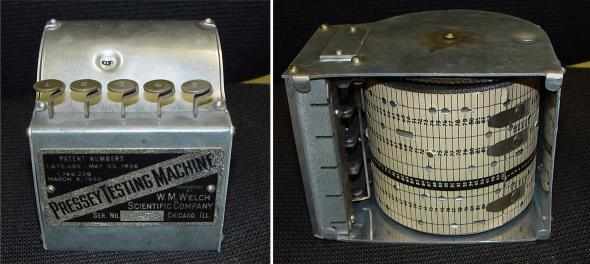
\includegraphics[scale=0.7]{imagens/pressey}
	\end{center}
	\legend{Fonte: \citeonline{pressey}}
	\label{fig:pressey}
\end{figure}

O uso da expressão ``pensamento computacional'', contudo, tem uma origem mais recente. O seu primeiro registro é observado no livro \textit{Mindstorms: Children, computers and powerful ideas}, da década de 1980, onde Seymour Papert discorre sobre a oportunidade trazida por computadores para o ensino de matemática. 

A popularização da expressão e o consequente interesse da comunidade acadêmica veio apenas com a publicação do artigo por \citeonline{wing2006}, no qual é proposto ``um conjunto de atitudes e habilidades universalmente aplicáveis'' assentadas na forma como cientistas da computação e programadores resolvem problemas.

Apesar do intenso debate despertado pelo artigo e do reconhecimento das questões e oportunidades educacionais implicadas no tema, o desenvolvimento de atividades e abordagens para sala de aula tem sido especialmente desafiador em face da parcial ou completa inexistência de um significado consensual para o conceito que seja adequado para este ambiente.

Essa indefinição tem tornado difícil o estabelecimento de formas mensuráveis de avaliar o progresso dos alunos e tem redundado na inviabilização do desenvolvimento de um currículo.

Na tentativa de preencher essa lacuna, um número significativo de conferências e congressos tem sido realizado ao redor do mundo, em especial nos Estados Unidos e na Europa, financiados em boa parte por secretarias de educação e grandes empresas de tecnologia. Ao mesmo tempo, desde da publicação de \citeonline{wing2006}, uma quantidade expressiva de artigos reportando experimentações em sala de aula tem sido publicados. 

O ponto de convergência desses debates tem sido a busca de uma definição clara sobre o significado desse conceito para o contexto da sala de aula, que ao mesmo tempo dialogue com particularidades e dificuldades pertinentes a esse ambiente.

Apesar da ausência de consenso, um conjunto numeroso de aplicações bem sucedidas tem apontado para algumas diretrizes.


















